
\begin{frame}{Introduction and definitions}
  \begin{itemize}
  \item Sub-differential (sub-gradient)
  \item Convex Conjugate
  \item Dual Norm
  \item Strong Convexity
  \item Smoothness
  \end{itemize}
\end{frame}

\begin{frame}{Convex Conjugate}
\begin{figure}
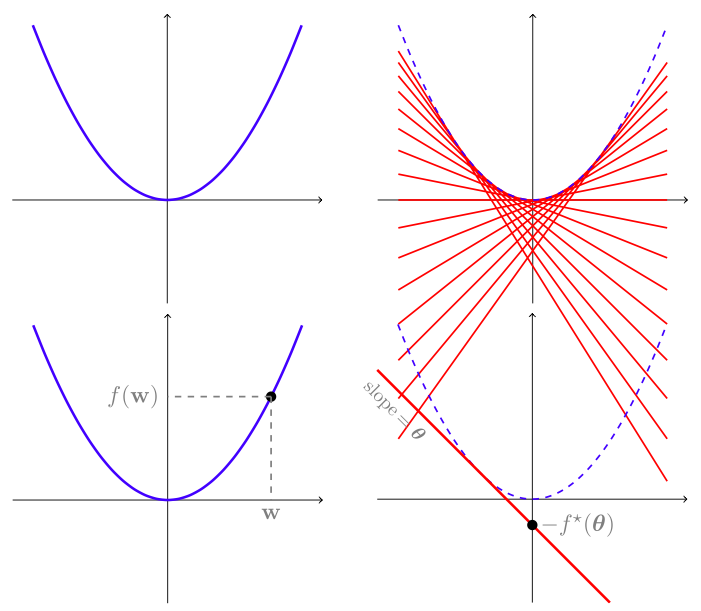
\includegraphics[scale=0.27]{images/fenchel.png}
\caption{From \cite{}}
\end{figure}
\end{frame}

\begin{frame}{Convex Conjugate}
\begin{align*}
\opt{\f}(\y) = \max_x \dotprod{\x}{\y} - \f(\x)
\end{align*}
\end{frame}

\begin{frame}{Dual Norm}
\begin{align*}
\opt{\f}(\y) = \max_x \dotprod{\x}{\y} - \f(\x)
\end{align*}
Fenchel conjugate of $\frac{\|\x\|^2}{2}$ is $\frac{\|\x\|_{*}^2}{2}$.
\end{frame}


\begin{frame}{Strong Convexity}
  Recall a function is convex if,
  \begin{align*} 
    \underbrace{\f(\x) + \dotprod{\grad \f(\x)}{\y-\x}}_{\text{the value at $\y$ of the tangent at $\x$}} \le \f(\y) \\
    \text{Rearranging, } \f(\x)-\f(\y) \le \dotprod{\grad \f(\x)} {\x-\y} \\
  \end{align*}
  A function is said to be $\beta$ strongly convex if,
  \begin{align*}
    \f(\x+\y) \ge \underbrace{\f(\x) + \dotprod{\grad \f(\x)}{\y}}_{\text{the value of the tangent}} +\frac{\beta}{2} \|\y\|^2
  \end{align*}
  Equivalently,
  \begin{align*}
    \f(\alpha \x +(1-\alpha)\y) \le \alpha \f(\x) + (1-\alpha)\f(\y) - \alpha(1-\alpha)\frac{\beta}{2} \|\y-\x\|^2
  \end{align*}
\end{frame}

\begin{frame}{Smoothness}
  A function is said to be $\beta$ smooth if,
  \begin{align*}
    \f(\x+\y) \le \f(\x) + \dotprod{\grad \f(\x)}{\y} +\frac{\beta}{2} \|\y\|^2
  \end{align*}
\end{frame}

\begin{frame}{Strong/Smoothness Duality}
  \begin{theorem}
    Assume $\f$ is closed and convex function. Then
    \begin{align*}
      \f \text{ is } \beta\text{-strongly convex} \iff \opt{\f} \text{ is } \frac{1}{\beta}\text{-smooth}
    \end{align*}
  \end{theorem}
\end{frame}

\begin{frame}{A Useful Lemma}
  \begin{lemma}
    If $\f$ is $\beta$ strong convex,
    \begin{align*}
      \sum_{i=1}^n \dotprod{v_i}{u} - f(u) \le \opt{\f}(v_{1:n}) \le \sum_{i=1}^n \dotprod{\grad \opt{\f}(v_{1:i-1})}{v_i} +\frac{1}{2\beta} \sum_{i=1}^n \|v_i\|^2
    \end{align*}
  \end{lemma}
  \begin{proof}
    Induction on the definition of smoothness.
  \end{proof}
\end{frame}

\begin{frame}{Follow the Regularized Leader}
  \begin{algorithmic}
    \Let{$\w_1$}{$\grad \opt{f}(0)$} 
    \For{$t=1$ ... $T$}
    \State Play $\w_t \in S$
    \State Receive $l_t$ and pick $v_t \in \partial l_t(w_t)$
    \State Update,
    \Let{$w_{t+1}$}{$\grad \opt{f}(-\eta \sum_{s=1}^{t} v_s)$}
    \EndFor
  \end{algorithmic}
\end{frame}

\begin{frame}{Generalized Regret Bound}
  \begin{align*}
    Regret(\w_1,\w_2,\cdots,\w_T,u) = \sum_{t=1}^T l_t(w_t) - \min_{u \in S} \sum_{t=1}^T l_t(u)
  \end{align*}
  \begin{theorem}
    \begin{align*}    
      Regret(\w_1,\w_2,\cdots,\w_T,u) \le \frac{\max_{u \in S} \f(u)}{\eta} + \frac{\eta V^2T}{2\beta}
    \end{align*}  
  \end{theorem}
\end{frame}

\begin{frame}
  \begin{proof}
    \begin{align*}    
      \sum_{t=1}^T l_t(w_t) - \sum_{t=1}^T l_t(u) \le \dotprod{v_t}{w_t - u} \tag{convexity} \\
      \sum_{t=1}^T \dotprod{v_t}{u} -f(u) \le \sum_{t=1}^T \dotprod{v_t}{w_t} +\frac{1}{2\beta} \sum_{t=1}^n \|v_t\|^2 \\
    \end{align*}  
  \end{proof}
\end{frame}

\begin{frame}{Rademacher Bounds}
  \begin{align*}
    \Rad(\F) = \E \left[ \sup_{f \in \F} \frac{1}{n}\sum_{i=1}^n \epsilon_i f(X_i) \right]
  \end{align*}
  \begin{align*}
    \X = \{ x : \|\|_{*} \le X \} \\
    \mathscr{W} = {w : f(w) \le f_{max}} \\
    \F = \{ x \mapsto \dotprod{w}{x} : w \in \mathscr{W} \} \\
    \Rad(\F) \le X\sqrt{\frac{2f_{max}}{\beta n}}
  \end{align*}
\end{frame}

\begin{frame}
  \begin{proof}
    \begin{align*}
      \sup_{w \in \mathscr{W}} \sum_{i=1}^n \dotprod{w}{\epsilon_i \lambda X_i} & \le \frac{\lambda^2}{2\beta}\sum_{i=1}^n \|\epsilon_i \lambda X_i\|_{*}^2 \\
      & + \sup_{w \in \mathscr{W}} f(w) \\
      & + \sum_{i=1}^n \dotprod{\grad \opt{f}(v_{1:i-1})}{\epsilon_i \lambda X_i} \\
      \Rad(\F) & \le \frac{\lambda X^2}{2\beta} + \frac{f_{max}}{n\lambda}
    \end{align*}
  \end{proof}
\end{frame}
